%! Author = shaji
%! Date = 06-Feb-23


\chapter{Predicate Invention}


\section{Spatial Area Map}
As shown in figure \ref{fig:8-area}, the surrounding area according to the reference object has been divided into 8 sub-areas.
This map both considers the distance and directions of the latent relation objects.


\begin{figure}
    \centering
    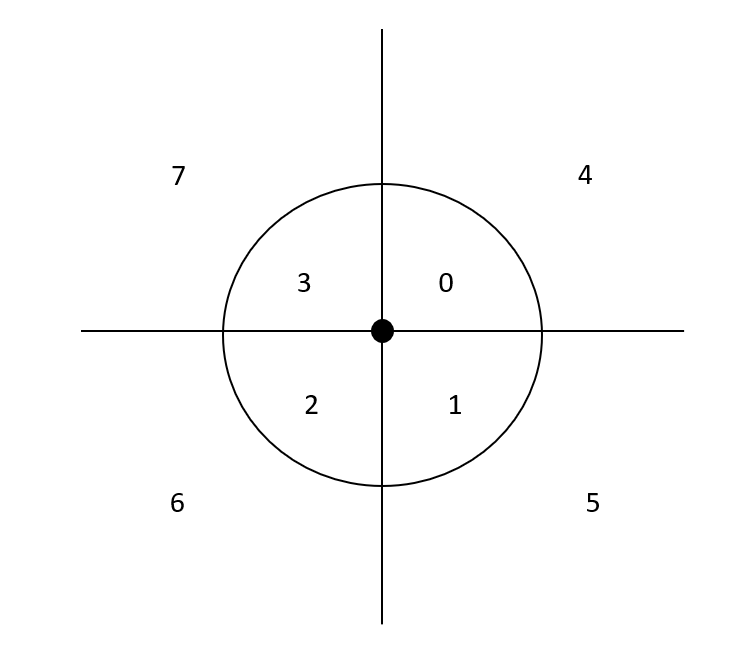
\includegraphics[width=\linewidth]{img/area_8}
    \caption{8-divide spatial area map with a clockwise naming.}
    \label{fig:8-area}
\end{figure}


\section{Inference}

\subsection{Clustering}
New predicate can be learned by clustering existed predicates.
One of the possible solution for \texttt{nearby} concept can be

\begin{align*}
    target(X,Y) &\leftarrow pred1(X,Y) \\
    pred1(X,Y) &\leftarrow atArea0(X,Y) \\
    pred1(X,Y) &\leftarrow atArea1(X,Y) \\
    pred1(X,Y) &\leftarrow atArea2(X,Y) \\
    pred1(X,Y) &\leftarrow atArea3(X,Y) \\
\end{align*}

Some of clauses generated from NSFR:
\begin{align*}
    target(X,Y) &\leftarrow atArea0(X,Y), atArea2(Y,X)  \\
    target(X,Y) &\leftarrow atArea1(X,Y),atArea3(Y,X) \\
    target(X,Y) &\leftarrow atArea1(X,Y) \\
    target(X,Y) &\leftarrow atArea2(X,Y) \\
    target(X,Y) &\leftarrow atArea4(X,Y),atArea6(Y,X) \\
    target(X,Y) &\leftarrow atArea5(X,Y),atArea7(Y,X) \\
    target(X,Y) &\leftarrow atArea5(X,Y) \\
    target(X,Y) &\leftarrow atArea6(X,Y) \\
    target(X,Y) &\leftarrow pred1(X,Y) \\
\end{align*}

Clauses generated from PI model:
\begin{align*}
    pred1(X,Y) &\leftarrow atArea0(Y,X), atArea2(X,Y) \\
    pred1(X,Y) &\leftarrow atArea1(Y,X),  atArea3(X,Y) \\
    pred1(X,Y) &\leftarrow atArea1(Y,X) \\
    pred1(X,Y) &\leftarrow atArea2(X,Y) \\
\end{align*}

We can use multi-step reasoning to conclude the target predicate.

A brief pipeline description of this work is shown in figure\ref{fig:pi_workflow}.
\begin{figure*}[ht]
    \centering
    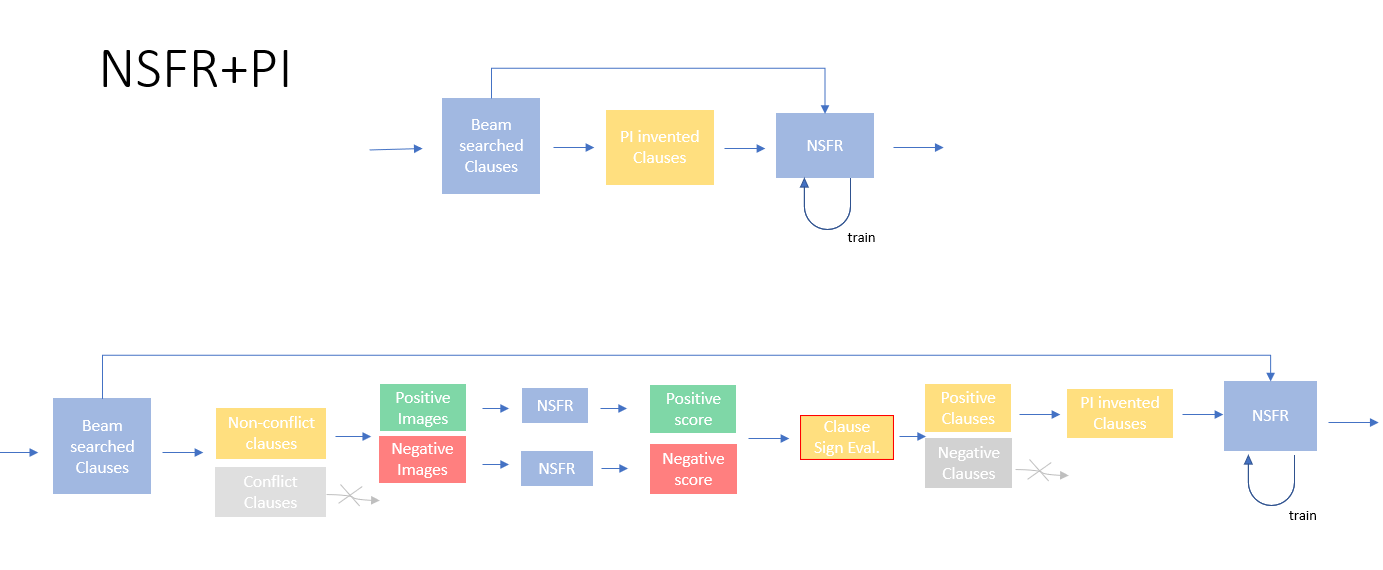
\includegraphics[width=\linewidth]{/img/pi_workflow}
    \caption{Pipeline of NSFR with PI module.}
    \label{fig:pi_workflow}
\end{figure*}


\begin{figure*}[H]
    \centering
    \begin{minipage}{.3\textwidth}
        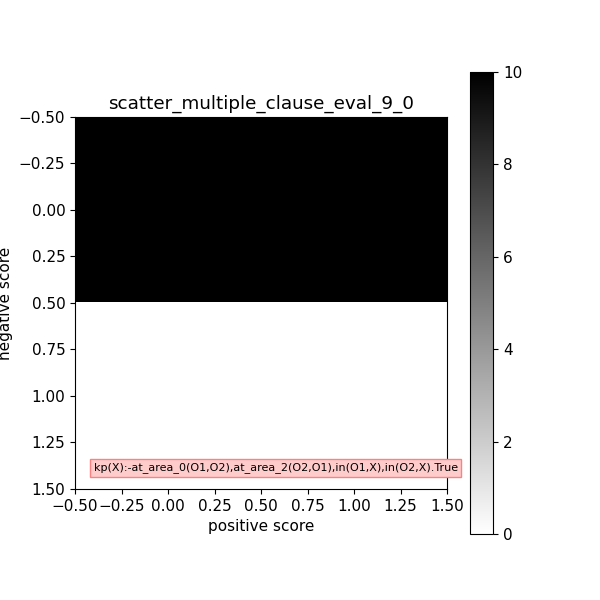
\includegraphics[width=\textwidth]{img/mce/mce-0}
        \caption{Caption}\label{label-a}
    \end{minipage}
    \begin{minipage}{.3\textwidth}
        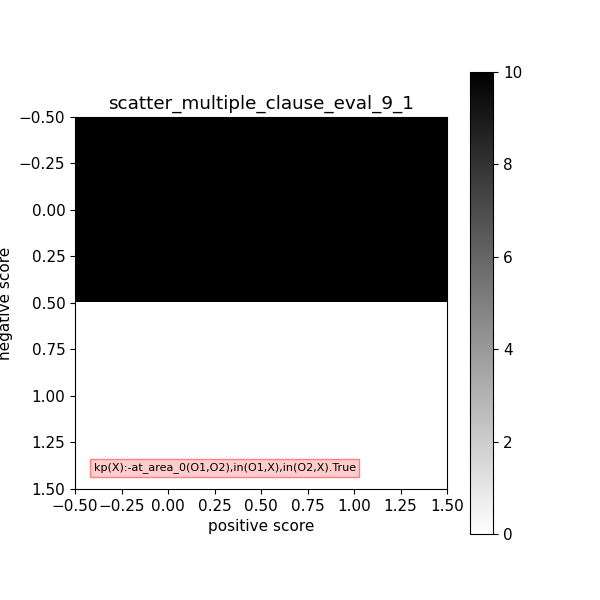
\includegraphics[width=\textwidth]{img/mce/mce-1}
        \caption{Caption}\label{label-b}
    \end{minipage}
    \begin{minipage}{.3\textwidth}
        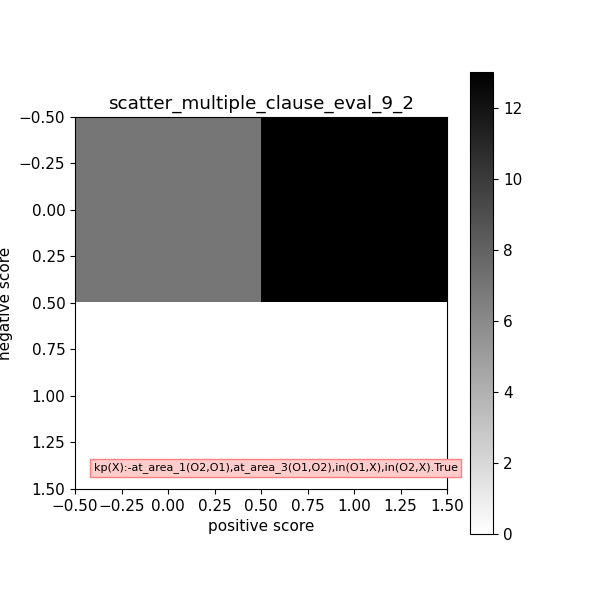
\includegraphics[width=\textwidth]{img/mce/mce-2}
        \caption{Caption}\label{label-c}
    \end{minipage}
    \begin{minipage}[b]{.3\textwidth}
        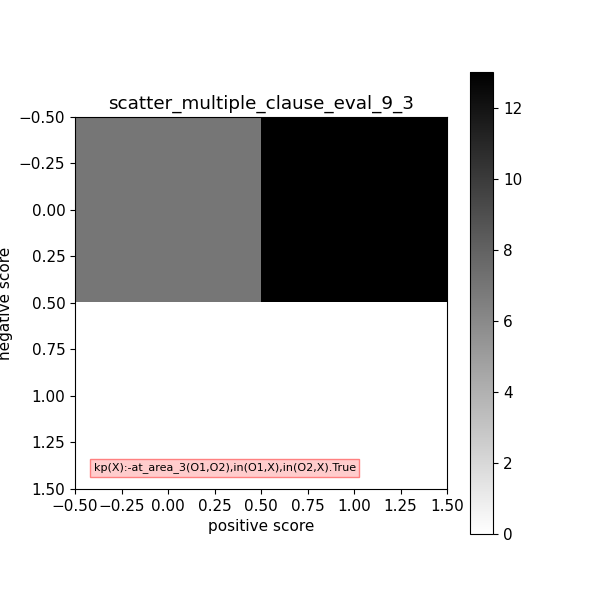
\includegraphics[width=\textwidth]{/img/mce/mce-3}
        \caption{Caption}\label{label-d}
    \end{minipage}
    \begin{minipage}[b]{.3\textwidth}
        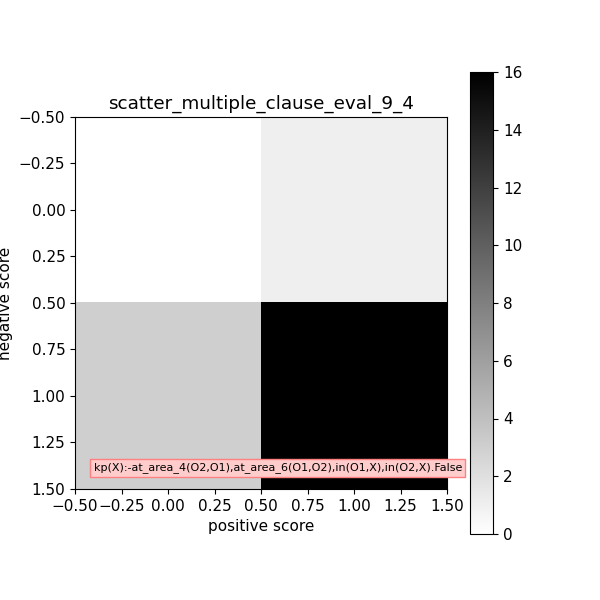
\includegraphics[width=\textwidth]{img/mce/mce-4}
        \caption{Caption}\label{label-e}
    \end{minipage}
    \begin{minipage}[b]{.3\textwidth}
        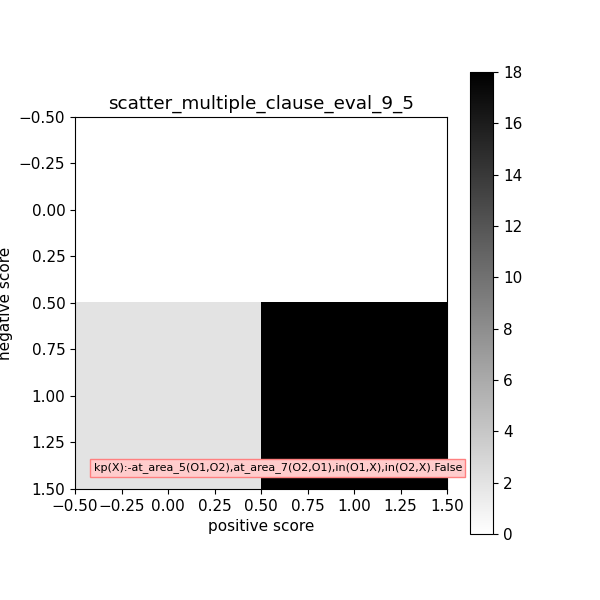
\includegraphics[width=\textwidth]{/img/mce/mce-5}
        \caption{Caption}\label{label-f}
    \end{minipage}
    \begin{minipage}[b]{.3\textwidth}
        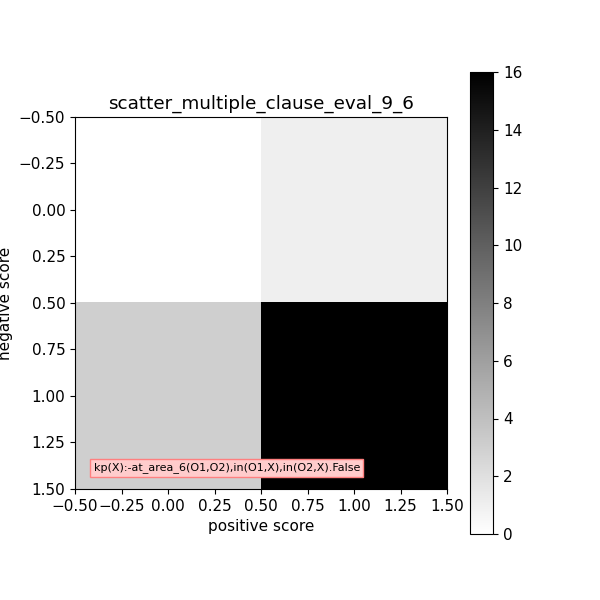
\includegraphics[width=\textwidth]{img/mce/mce-6}
        \caption{Caption}\label{label-g}
    \end{minipage}
    \begin{minipage}[b]{.3\textwidth}
        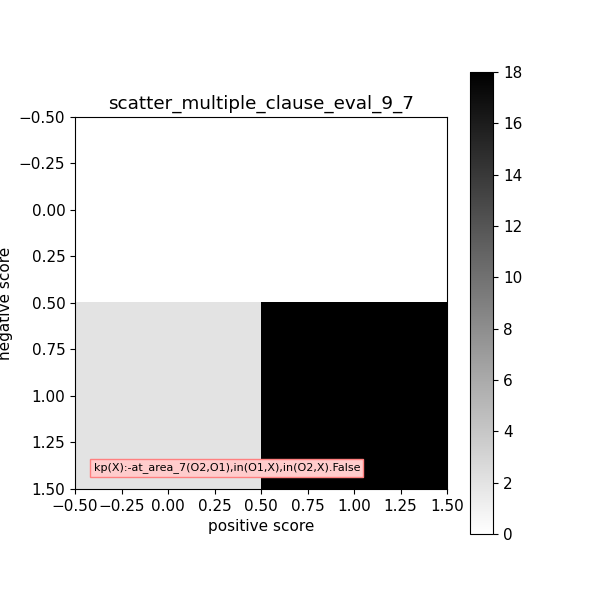
\includegraphics[width=\textwidth]{img/mce/mce-7}
        \caption{Caption}\label{label-h}
    \end{minipage}
    \begin{minipage}[b]{.3\textwidth}
        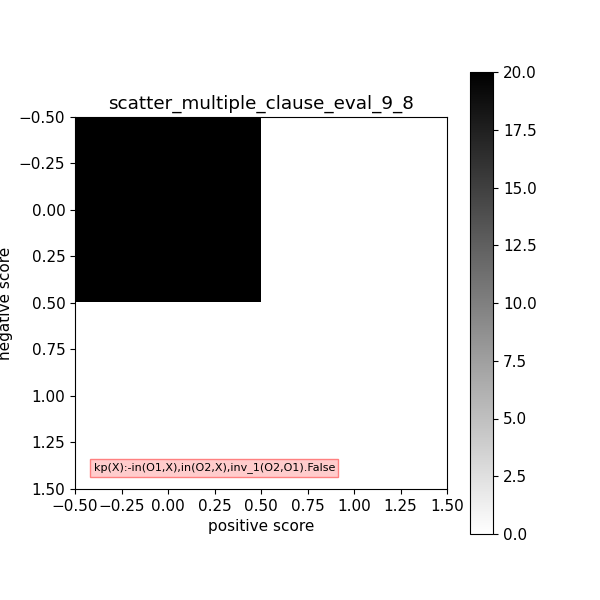
\includegraphics[width=\textwidth]{img/mce/mce-8}
        \caption{Caption}\label{label-i}
    \end{minipage}
    \caption{Pipeline of NSFR with PI module.}
    \label{fig:mce}
\end{figure*}



\begin{table}
    \caption{Predict Result}
    \label{tab:nearby-pi-result}
    \begin{tabular}{ccl}
        \toprule
        Dataset   & Accuracy & Number of Images \\
        \midrule
        Train     & 1.0      & 40               \\
        Test      & 1.0      & 40               \\
        Valuation & 1.0      & 40               \\
        \bottomrule
    \end{tabular}
\end{table}

\subsection{Chaining}
This paper\cite{dILP} supports predicate invention.


